\documentclass[tikz,border=6pt]{standalone}
\usepackage{amsmath}
\usetikzlibrary{positioning}

\begin{document}
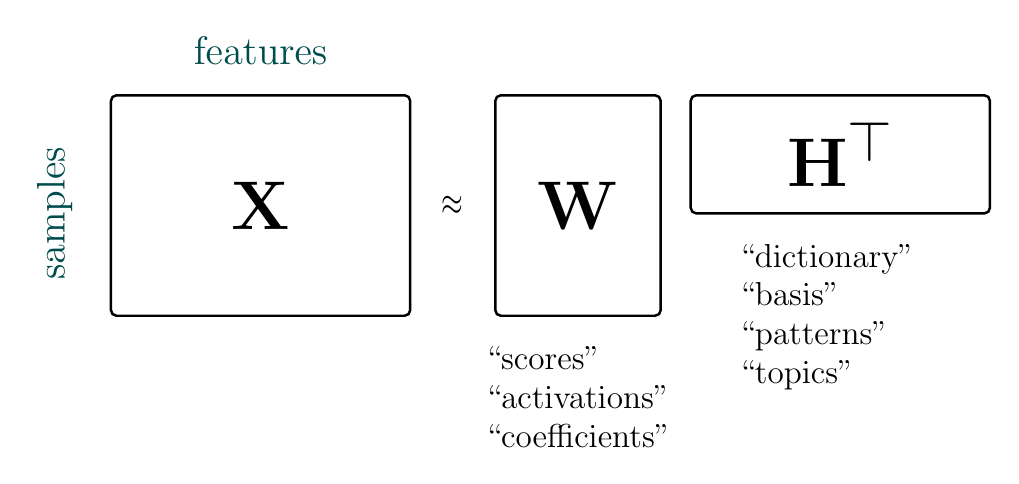
\begin{tikzpicture}[
  matrixbox/.style={
    draw,
    rounded corners=2pt,
    line width=0.9pt,
    align=center
  },
  xbox/.style={
    matrixbox,
    minimum width=3.8cm,
    minimum height=2.8cm
  },
  wbox/.style={
    matrixbox,
    minimum width=2.1cm,
    minimum height=2.8cm
  },
  htbox/.style={
    matrixbox,
    minimum width=3.8cm,
    minimum height=1.5cm
  },
  approx/.style={font=\Large, xscale=0.7},
  dimlabel/.style={font=\small},
  axislabel/.style={font=\Large, text=teal!60!black},
  desc/.style={font=\large, align=left},
  matlabel/.style={font=\fontsize{28}{32}\selectfont}
]

\node[xbox, matlabel] (x) {$\mathbf{X}$};
\node[approx, right=0.3cm of x] (approx) {$\approx$};
\node[wbox, right=0.3cm of approx, matlabel] (w) {$\mathbf{W}$};
\node[htbox, right=0.35cm of w.north east, anchor=north west, matlabel] (ht) {$\mathbf{H}^{\top}$};

\node[axislabel, above=0.25cm of x] {features};
\node[axislabel, rotate=90] at ([xshift=-0.7cm,yshift=-0.1cm]x.west) {samples};

\node[desc, anchor=north] at ([yshift=-0.25cm]w.south) {``scores''\\``activations''\\``coefficients''};
\node[desc, anchor=north west] at ([xshift=0.5cm,yshift=-0.25cm]ht.south west) {``dictionary''\\``basis''\\``patterns''\\``topics''};

\end{tikzpicture}
\end{document}
